\documentclass[10pt,a4paper]{report}
\usepackage[utf8]{inputenc}
\usepackage{amsmath}
\usepackage{amsfonts}
\usepackage{amssymb}
\usepackage{graphicx}
\usepackage{hyperref}
\usepackage{bm}
\usepackage{gensymb}
\usepackage[left=2cm,right=2cm,top=2cm,bottom=2cm]{geometry}
\setlength\parindent{0pt}
\graphicspath{{./images/}}
\begin{document}


\textbf{Additional Project 2.1: The Diffusion Equation}
\thispagestyle{empty}

\newpage

\subsection*{Question 1}

Rearranging the equation for F(x,t):

\begin{equation*}
F(x,t)=\frac{\theta(x,t)- \theta_0}{\theta_1 - \theta_0}  
\end{equation*}

The RHS is a dimensionless quantity, hence F is dimensionless, for all x,t. Hence F must be a function of some dimensionless variables. The problem contains 3 variables; K, x, and t, with $[K]=L^2T^{-1}$, $[x]=L$, $[t]=T$. Since we can only add quantities of the same dimension, the simplest relation we can have is a power law. Letting  $x^a t^b K^c$ be dimensionless, we find any dimensionless variable is some power of $\varepsilon = \frac{x}{\sqrt{Kt}}$, so we have $F(x,t)=f(\varepsilon)$ generally.\par

\begin{equation*}
\theta_t=K\theta_{xx} \quad \text{and} \quad \theta(x,t)=\theta_0+(\theta_1 - \theta_0)F(x,t)
\end{equation*}

imply 

\begin{equation*}
F_t=KF_{xx}
\end{equation*}

and we have new boundary conditions

\begin{equation*}
F(x,0)=0, \quad F(0,t)=1 \quad \text{for } t>0
\end{equation*}

and, as $x \rightarrow \infty$, either

\begin{equation*}
(a) \quad \frac{\partial F}{\partial x}(x,t) \rightarrow 0 \quad \text{or} \quad (b)\quad F(x,t) \rightarrow 0
\end{equation*}

Now 

\begin{equation} \label{*}
\frac{\partial F}{\partial t} = \frac{df}{d\varepsilon}\frac{\partial \varepsilon}{\partial t} = 
\frac{df}{d\varepsilon}\frac{(-x)}{2K^{1/2}t^{4/2}} \quad \text{and similarly} \quad \frac{\partial F}{\partial x}=\frac{df}{d\varepsilon}\frac{1}{\sqrt{Kt}} \quad \text{and} \quad  \frac{\partial^2 F}{\partial x^2}=\frac{d^2f}{d\varepsilon^2}\frac{1}{Kt} \tag{*}
\end{equation}

giving

\begin{equation*}
(\frac{-\varepsilon}{2})\frac{df}{d\varepsilon} = \frac{d^2f}{d\varepsilon^2}
\end{equation*}

Integrating we get 

\begin{equation*}
\frac{df}{d\varepsilon} = C_1exp(-\frac{\varepsilon^2}{4})
\end{equation*}

and by FTC we get 

\begin{equation*}
f(\varepsilon) = C_2\int_{\varepsilon/2}^{\infty}exp(-u^2)du + C_3
\end{equation*}

$F(x,0)=0 \Rightarrow f(\varepsilon) \rightarrow 0$ as $\varepsilon \rightarrow \infty$ giving $C_3=0$. $F(0,t)=1$ for $t>0 \Rightarrow f(0)=1 \Rightarrow C_2=\frac{2}{\sqrt{\pi}}$. Hence

\begin{equation*}
f(\varepsilon) = \frac{2}{\sqrt{\pi}} \int_{\varepsilon/2}^{\infty}exp(-u^2)du = erfc(\varepsilon/2)
\end{equation*}

as required. Note we did not use conditions (a) or (b), but the solution satisfies both (a) and (b) by (*), as $x\rightarrow\infty\Rightarrow\varepsilon\rightarrow\infty$


\subsection*{Question 2}

i) First consider the fixed-endpoint temperature problem. Write $\hat{U}(X,T)=U(X,T)-U_s(X)$, where $U_s(X)$ is the steady state solution $1-X$, to convert the problem into one with homogeneous boundary conditions. We get

\begin{equation*}
\hat{U}_T=\hat{U}_{XX} 
\end{equation*}
\begin{equation*}
\hat{U}(0,T)=0 \quad \text{for }T>0
\end{equation*}
\begin{equation*}
\hat{U}(1,T)=0 \quad \text{for }T>0
\end{equation*}
\begin{equation*}
\hat{U}(X,0)=X-1 \tag{**}
\end{equation*}

Now separate variables. Write $\hat{U}(X,T)=A(X)B(T)$. Plugging into the ODE, we get

\begin{equation*}
\frac{\dot{B}}{B}=\frac{A''}{A}
\end{equation*}

where the LHS is a function only of T, and the RHS of only X, hence equal to a negative constant $-\lambda$ (the negative is required, else impossible for A(1) to be 0 below). Thus 

\begin{equation*}
A(X)=C_1sin(\sqrt{\lambda}X)+C_2cos(\sqrt{\lambda}X)
\end{equation*}

Using the boundary conditions, $A(0)=0\Rightarrow C_2=0$. Also $A(1)=0\Rightarrow sin(\sqrt{\lambda})=0 \Rightarrow \lambda=n^2\pi^2$ for some $n\in\mathbb{N}$. This gives

\begin{equation*}
A_n(X)=sin(n\pi X) \quad \text{and} \quad B_n(T)=e^{-n^2\pi^2 T}
\end{equation*}

So the general solution is,

\begin{equation*}
\hat{U}(X,T)=\sum_{n\geq 1} c_n sin(n\pi X) e^{-n^2\pi^2 T}
\end{equation*}

We use the T=0 condition, along with orthogonality of eigenfunctions to calculate the $c_n=-\frac{2}{\pi n}$. Thus 

\begin{equation*}
U_{fixed}(X,T)=1-X-\frac{2}{\pi}\sum_{n\geq 1} \frac{1}{n}sin(n\pi X) e^{-n^2\pi^2 T}
\end{equation*}

\vspace{1cm}

ii) For the insulated end problem, we proceed as above, but set our steady state solution to $U_s(X)=1$, giving (**) except $\hat{U}(X,0)=-1$ and $\hat{U}_X(1,T)=0$ for $T>0$. Following the same method, we get

\begin{equation*}
A(X)=C_1sin(\sqrt{\lambda}X)+C_2cos(\sqrt{\lambda}X)
\end{equation*}

Using the boundary conditions, $A(0)=0\Rightarrow C_2=0$. Also $A_X(1)=0\Rightarrow cos(\sqrt{\lambda})=0 \Rightarrow \lambda=(n+1/2)^2\pi^2$ for $n=1,2,3...$. Thus get 

\begin{equation*}
A_n(X)=sin((n+1/2)\pi X) \quad \text{and} \quad B_n(T)=e^{-(n+1/2)^2\pi^2 T}
\end{equation*}

and general solution

\begin{equation*}
\hat{U}(X,T)=\sum_{n\geq 0} c_n sin((n+\frac{1}{2})\pi X) e^{-(n+1/2)^2\pi^2 T}
\end{equation*}

and again, using the T=0 condition and orthogonality gives $c_n=-\frac{2}{\pi(n+1/2)}$. So have, rewriting from n=1,

\begin{equation*}
U_{insulated}(X,T)=1-\frac{2}{\pi}\sum_{n\geq 1} \frac{1}{n-1/2}sin((n-\frac{1}{2})\pi X) e^{-(n-1/2)^2\pi^2 T}
\end{equation*}

\subsection*{Programming Task}

The script $evaluateanalytic$, found on page 11 evaluates the analytic solutions $U_{fixed}$ and $U_{insulated}$, up to n=25. We do the same for the derivatives in $evaluateanalyticflux.m$ (see page 12). This should be sufficient, since the error $E_{fixed}$ very crudely satisfies

\begin{equation*}
\begin{split}
|E_{fixed}| & =  |\sum_{n\geq 26} \frac{1}{n}sin(n\pi X) e^{-n^2\pi^2 T}| \\
 & \leq \sum_{n\geq 26} |\frac{1}{n}sin(n\pi X) e^{-n^2\pi^2 T}|\\
 & \leq \sum_{n\geq 26} e^{-n^2\pi^2 T}\\
 & \leq \sum_{n\geq 26} e^{-n\pi^2 T}\\
 & = e^{-26\pi^2T}\frac{1}{1-e^{-\pi^2T}}\\
 & \leq 2.36\text{x}10^{-7} \quad \text{for } T\geq 0.0625 
\end{split} 
\end{equation*}

Similarly, we get the same bound for $E_{insulated}$, and for the derivatives. This error should be sufficiently small, since we are considering a function varying between 0 and 1. We will confirm whether this accuracy is suitable when doing Q3.

\begin{verbatim}

>> evaluateanalytic.m %with T=0.25

\end{verbatim}

\begin{table}[h]
\centering
\begin{tabular}{|l|l|l|l|}
\hline
\textbf{X} & $U_{fixed}$  & $U_{insulated}$ & $U_{semi-inf}$ \\ \hline
0.000      & 1.000     & 1.000        & 1.000       \\ \hline
0.125      & 0.854     & 0.865        & 0.860       \\ \hline
0.250      & 0.712     & 0.736        & 0.724       \\ \hline
0.375      & 0.575     & 0.617        & 0.596       \\ \hline
0.500      & 0.446     & 0.513        & 0.480       \\ \hline
0.625      & 0.325     & 0.428        & 0.377       \\ \hline
0.750      & 0.212     & 0.366        & 0.289       \\ \hline
0.875      & 0.104     & 0.327        & 0.216       \\ \hline
1.000      & -6.61E-18 & 0.315        & 0.157       \\ \hline
\end{tabular}
\caption{Analytical Solutions at T=0.25}
\end{table}


\begin{verbatim}

>> evaluateanalyticflux 

\end{verbatim}

\begin{figure}[h]
\centering
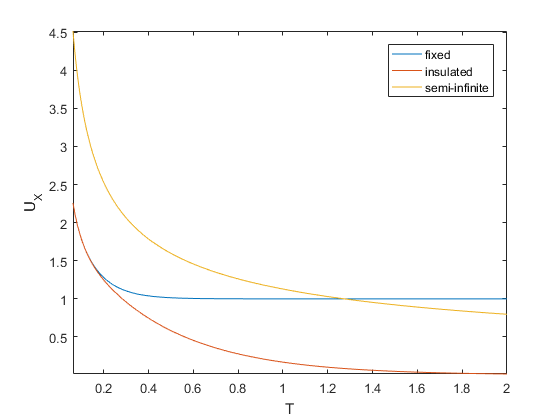
\includegraphics{flux}
\caption{Flux at $X=0$}
\end{figure}

\newpage

\begin{figure}[ht]
\begin{minipage}[b]{0.5\linewidth}
\centering
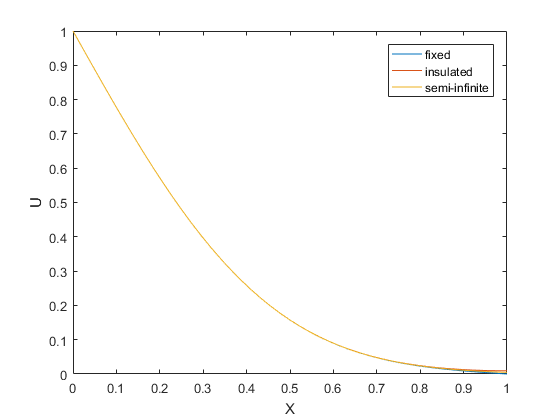
\includegraphics[width=\textwidth]{anal00625}
\caption{Output of with $T=0.0625$}
\end{minipage}
\hspace{0.5cm}
\begin{minipage}[b]{0.5\linewidth}
\centering
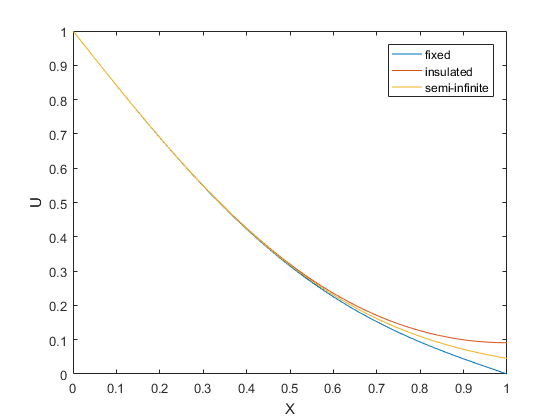
\includegraphics[width=\textwidth]{anal0125}
\caption{Output with $T=0.125$}
\end{minipage}
\end{figure}

\begin{figure}[ht]
\begin{minipage}[b]{0.5\linewidth}
\centering
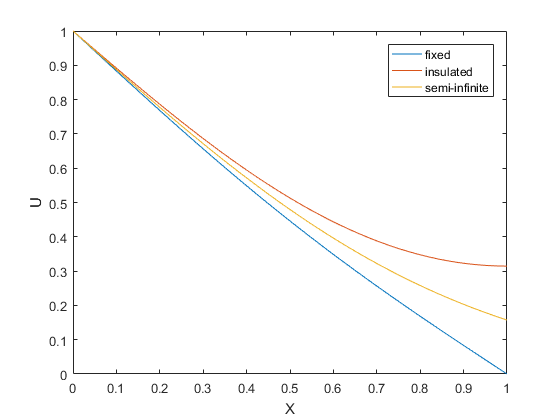
\includegraphics[width=\textwidth]{anal025}
\caption{Output with $T=0.25$}
\end{minipage}
\hspace{0.5cm}
\begin{minipage}[b]{0.5\linewidth}
\centering
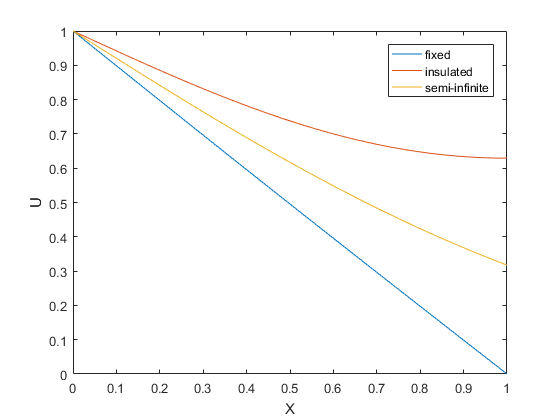
\includegraphics[width=\textwidth]{anal05}
\caption{Output with $T=0.5$}
\end{minipage}
\end{figure}

\begin{figure}[ht]
\begin{minipage}[b]{0.5\linewidth}
\centering
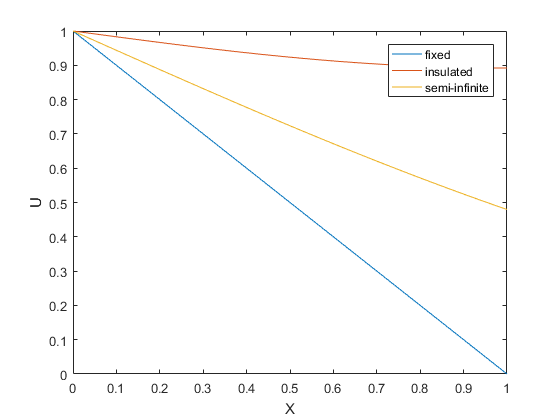
\includegraphics[width=\textwidth]{anal1}
\caption{Output with $T=1$}
\end{minipage}
\hspace{0.5cm}
\begin{minipage}[b]{0.5\linewidth}
\centering
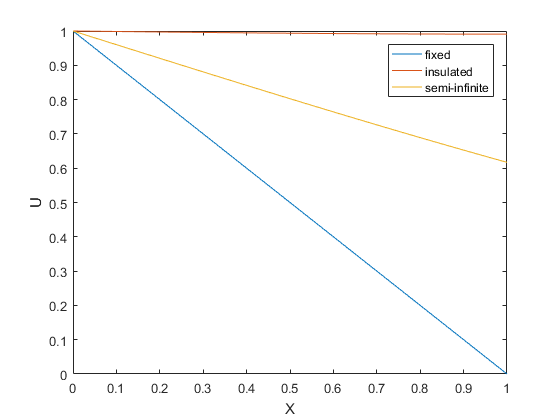
\includegraphics[width=\textwidth]{anal2}
\caption{Output with $T=2$}
\end{minipage}
\end{figure}





\newpage 

For all 3 solutions, the $U(X,0)=0$ for $0<X<1$ and $U(0,T)=1$ initial and boundary conditions define the behaviour for small time; we get a sharp continuous drop from 1 to 0 in the functions value over a small change in X. This can be seen in figure 1, but is more clear in figure 7; the flux tends to $\infty$ as $T \rightarrow 0$ in all 3 cases.
\vspace{0.5cm}

The long term behaviour is determined by the boundary conditions at $X=1$ or as $X\rightarrow\infty$. The fixed boundary condition solution converges quite quickly to its "steady state" solution $1-X$, since the infinite sum $\rightarrow 0$ as $T\rightarrow\infty$ due to the negative exponentials. The insulated boundary condition solution is similar, but converges slower to $1$, due to the $n-1/2$ (as opposed to n) eigenvalues in the exponentials. \par
\vspace{0.5cm}

The semi-infinite solution does not have any significant behaviour at X=1, but rather is controlled as $X\rightarrow\infty$, and shares properties of both other solutions at $\infty$ in that both $U$ and $U_X$ tend to 0 there. As T increases, the graph shifts up, since the argument $\varepsilon/2$, of erfc, is inversely proportional to $\sqrt{T}$, with the solution tending to 1 for fixed X as $T\rightarrow\infty$.
\vspace{0.5cm}

Physically, the initial high flux makes sense, since we have a very high temperature at one end, adjacent to 0K. The evolution in time can be thought of as heat "travelling down the bar", until the bar eventually reaches its long term behaviour. In the fixed case, we have some "hot" end, and some "cold" end and one would expect a linear decrease in temperature along the rod, as we observe. For the insulated case, since we have no heat flux out of the system, we would expect the whole rod to eventually become the same temperature, 1. This intuition is easily extended to the infinite case.

\newpage

\subsection*{Question 3}

The script $NumericalScheme.m$, found on page 13 runs the given numerical scheme, by calculating all $U_n^m$ for fixed m, before moving onto the next n. Note

\begin{equation*}
U(X,0) = 0 \quad \text{for} \quad 0<X<1 \quad  \Rightarrow \quad  U_n^0 = 0 \quad \text{for} \quad n \neq 0
\end{equation*}

\begin{equation*}
U(0,T) = 1 \quad \text{for} \quad T> 0 \quad  \Rightarrow \quad  U_0^m = 1 \quad \text{for} \quad m \neq 0
\end{equation*}

and combining these conditions at $X=T=0$ gives a best approximation $U_0^0=0.5$. To implement the derivative boundary condition, \textbf{consider the symmetric central difference in space at X=1 (despite U only being defined on $0<X<1$)}. 

\begin{equation*}
U_X(1,T) = \frac{U(1+\delta X,T) - U(1-\delta X,T)}{2\delta X} + O(\delta X) = 0
\end{equation*}

Hence, as $\delta X \to 0$

\begin{equation*}
U(1+\delta X,T) = U(1-\delta X,T) \quad \text{for} \quad T>0 \quad \Rightarrow \quad U_{N+1}^m=U_{N-1}^m
\end{equation*}

\vspace{2cm}



(i) The script $q3i.m$, found on page 13, produces the following output for varying T. Note we define the error $E=U_{numerical}-U_{analytic}$
\begin{table}[h]
\begin{minipage}[b]{0.5\linewidth}
\centering

\begin{tabular}{|l|l|l|l|}
\hline
X & $U_{numerical}$ & $U_{analytic}$ & E \\ \hline
0.000      & 1.000       & 1.000  & 0.000E+00            \\ \hline
0.125      & 0.804       & 0.803  & 9.071E-04            \\ \hline
0.250      & 0.618       & 0.618  & 7.831E-04            \\ \hline
0.375      & 0.455       & 0.454  & 6.104E-04            \\ \hline
0.500      & 0.319       & 0.320  & -1.315E-03           \\ \hline
0.625      & 0.214       & 0.217  & -2.964E-03           \\ \hline
0.750      & 0.141       & 0.146  & -5.012E-03           \\ \hline
0.875      & 0.098       & 0.105  & -6.484E-03           \\ \hline
1.000      & 0.084       & 0.091  & -6.803E-03           \\ \hline
\end{tabular}

\caption{Output with $T=0.125$}
\end{minipage}
\hspace{0.5cm}
\begin{minipage}[b]{0.5\linewidth}
\centering
\begin{tabular}{|l|l|l|l|}
\hline
X & $U_{numerical}$ & $U_{analytic}$ & E \\ \hline
0.000      & 1.000       & 1.000  & 0.000E+00            \\ \hline
0.125      & 0.865       & 0.865  & -9.164E-05           \\ \hline
0.250      & 0.735       & 0.736  & -3.187E-04           \\ \hline
0.375      & 0.616       & 0.617  & -5.147E-04           \\ \hline
0.500      & 0.512       & 0.513  & -9.898E-04           \\ \hline
0.625      & 0.427       & 0.428  & -1.307E-03           \\ \hline
0.750      & 0.364       & 0.366  & -1.817E-03           \\ \hline
0.875      & 0.325       & 0.327  & -1.989E-03           \\ \hline
1.000      & 0.312       & 0.315  & -2.201E-03           \\ \hline
\end{tabular}
\caption{Output with $T=0.25$}
\end{minipage}
\end{table}

\begin{table}[h]
\begin{minipage}[b]{0.5\linewidth}
\centering

\begin{tabular}{|l|l|l|l|}
\hline
X & $U_{numerical}$ & $U_{analytic}$ & E \\ \hline
0.000      & 1.000       & 1.000  & 0.000E+00            \\ \hline
0.125      & 0.928       & 0.928  & 1.156E-04            \\ \hline
0.250      & 0.858       & 0.858  & 1.995E-04            \\ \hline
0.375      & 0.794       & 0.794  & 3.274E-04            \\ \hline
0.500      & 0.738       & 0.738  & 3.657E-04            \\ \hline
0.625      & 0.692       & 0.692  & 4.860E-04            \\ \hline
0.750      & 0.658       & 0.657  & 4.739E-04            \\ \hline
0.875      & 0.637       & 0.636  & 5.701E-04            \\ \hline
1.000      & 0.630       & 0.629  & 5.112E-04            \\ \hline
\end{tabular}

\caption{Output with $T=0.5$}
\end{minipage}
\hspace{0.5cm}
\begin{minipage}[b]{0.5\linewidth}
\centering
\begin{tabular}{|l|l|l|l|}
\hline
X & $U_{numerical}$ & $U_{analytic}$ & E \\ \hline
0.000      & 1.000       & 1.000  & 0.000E+00            \\ \hline
0.125      & 0.979       & 0.979  & 2.010E-04            \\ \hline
0.250      & 0.959       & 0.959  & 3.865E-04            \\ \hline
0.375      & 0.941       & 0.940  & 5.723E-04            \\ \hline
0.500      & 0.924       & 0.924  & 7.141E-04            \\ \hline
0.625      & 0.911       & 0.910  & 8.565E-04            \\ \hline
0.750      & 0.901       & 0.900  & 9.331E-04            \\ \hline
0.875      & 0.895       & 0.894  & 1.010E-03            \\ \hline
1.000      & 0.893       & 0.892  & 1.010E-03            \\ \hline
\end{tabular}
\caption{Output with $T=1$}
\end{minipage}
\end{table}


(ii) The script $q3ii.m$, found on page 14, produces the following figures when run with different T, N=8, C=1/2.

\newpage

\begin{figure}[ht]
\begin{minipage}[b]{0.5\linewidth}
\centering
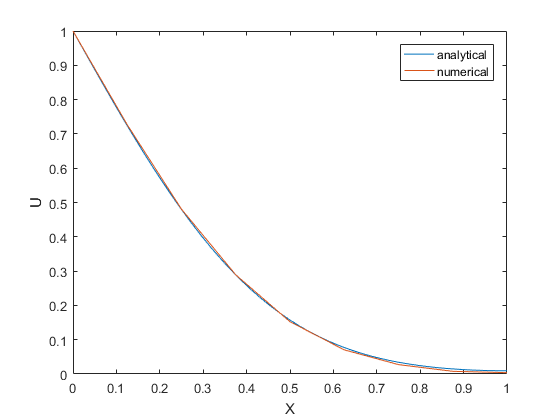
\includegraphics[width=\textwidth]{3ii00625}
\caption{Output with $T=0.0625$}
\end{minipage}
\hspace{0.5cm}
\begin{minipage}[b]{0.5\linewidth}
\centering
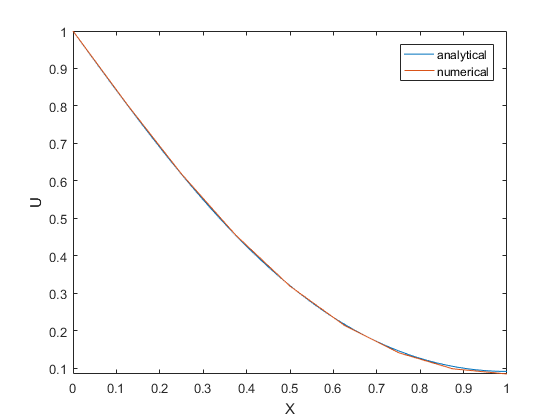
\includegraphics[width=\textwidth]{3ii0125}
\caption{Output with $T=0.125$}
\end{minipage}
\end{figure}

\begin{figure}[ht]
\begin{minipage}[b]{0.5\linewidth}
\centering
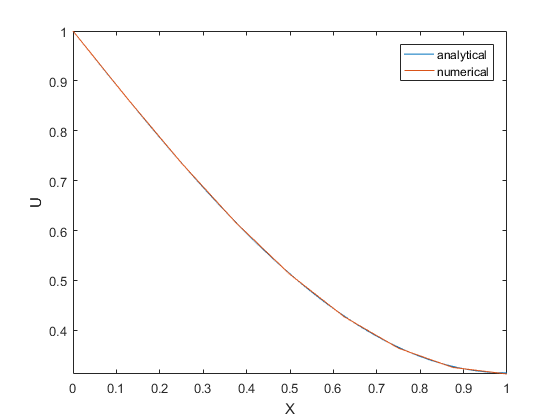
\includegraphics[width=\textwidth]{3ii025}
\caption{Output with $T=0.25$}
\end{minipage}
\hspace{0.5cm}
\begin{minipage}[b]{0.5\linewidth}
\centering
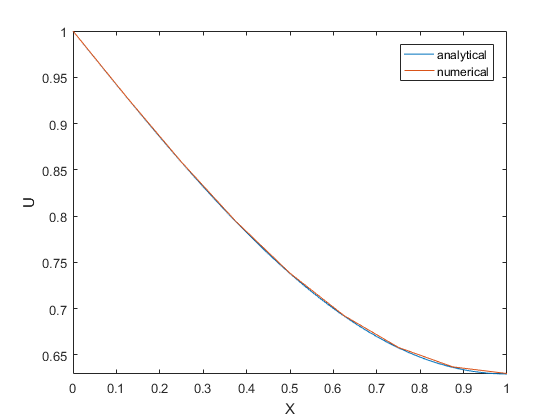
\includegraphics[width=\textwidth]{3ii05}
\caption{Output with $T=0.5$}
\end{minipage}
\end{figure}

\begin{figure}[ht]
\begin{minipage}[b]{0.5\linewidth}
\centering
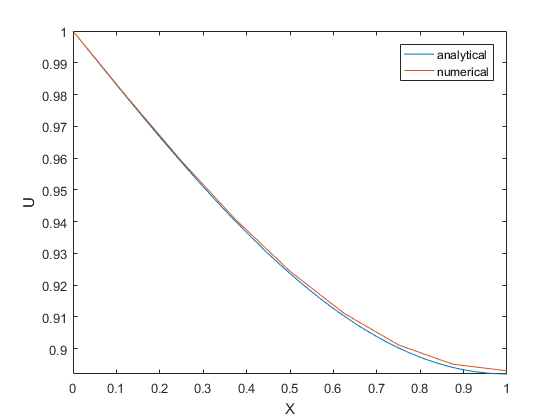
\includegraphics[width=\textwidth]{3ii1}
\caption{Output with $T=1$}
\end{minipage}
\hspace{0.5cm}
\begin{minipage}[b]{0.5\linewidth}
\centering
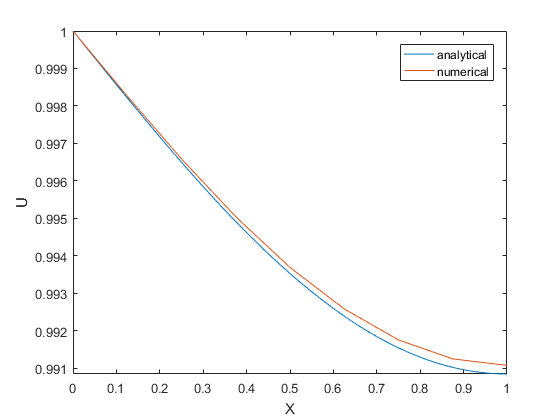
\includegraphics[width=\textwidth]{3ii2}
\caption{Output with $T=2$}
\end{minipage}
\end{figure}

\newpage

\subsubsection{Stability}

We run the script $NumericalScheme.m$ for $N=8$,$16$,$32$, $C=\frac{1}{12}$,$\frac{1}{6}$,$\frac{1}{3},\frac{1}{2}$,$\frac{2}{3}$ and 1, and observe stability in all cases but $C=\frac{2}{3}$ or 1. An example can be seen in figure 14. The instability manifests as oscillations growing in magnitude rapidly.

\begin{figure}[h]
\centering
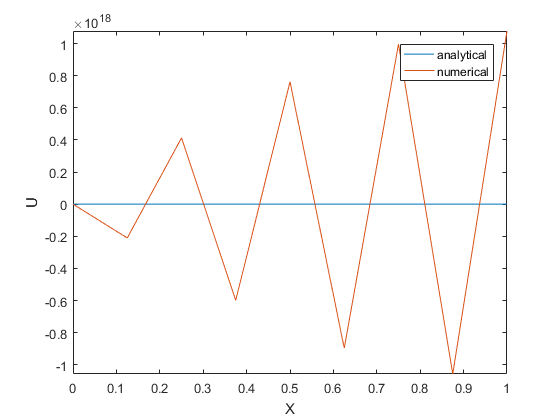
\includegraphics[width=10cm]{unstable}
\caption{Output of $q3ii.m$ with N=8, C=2/3, T=1}
\end{figure}

The data seems to suggest the scheme is stable for $C\leq\frac{1}{2}$ and unstable otherwise. This is in fact true, and can be shown by "Von Neumann Stability Analysis"  \footnote{
See \url{https://en.wikipedia.org/wiki/Von_Neumann_stability_analysis}, in particular, subsection "Illustration of the Method". Date Accessed 30/12/18}
; a method involving taking the fourier series of the round off errors, defined as 
  $\epsilon_n^m = N_n^m - U_n^m$ where $N_n^m$ is the exact solution to the difference equation. We then bound the amplification factor G such that 
  
\begin{equation*} 
|G| \equiv |\frac{\epsilon_n^{m+1}}{\epsilon_n^m}| \leq 1
\end{equation*}

This is equivalent to, for fixed $\delta X$, a sufficiently small $\delta T$ is needed for stability; $\delta T$ must satisfy

\begin{equation*}
\delta T \leq \frac{1}{2}(\delta X)^2
\end{equation*}

\subsubsection{Accuracy}

We can see from figures 8-13 that when the numerical scheme is stable it seems to be a good approximation to the solution at all times, with error maximised at T=2. We therefore consider errors at T=2 within this section. Note that at this time, the calculation for the error in the analytical solution through summing finite terms is of order $10^{-223}$ so we need not consider it.\par
\vspace{0.5cm}
To determine the theoretical accuracy of the scheme, we have;
\begin{align*}
(19) \quad &\Rightarrow \quad U_T(X,T)+O(\delta T)=\frac{U(X,T+\delta T)-U(X,T)}{\delta T}\\
(20) \quad &\Rightarrow \quad U_{XX}(X,T)+O((\delta X)^2)=\frac{U(X+\delta X,T)-2U(X,T)+U(X-\delta X,T)}{(\delta X)^2}
\end{align*}

and equating gives an error $E_n^m=O(\delta T)+O((\delta X)^2)$, and hence as $\delta X$ and $\delta T \rightarrow 0$, $E_n^m \approx A(\delta X)^2 + B(\delta T)$ for some constants A and B depending on various other factors (including the time we take the error at). We can test whether this is the case in our implementation by fixing say $\delta T$, and checking whether the differences between errors for changing $\delta X$ are quadratic. A similar approach can be applied to check the errors for fixed $\delta X$ and changing $\delta T$ are linear. Note the error itself for fixed $\delta X$ will not tend to 0, and will rather tend to a non zero limit as $\delta T$ tends to 0 due to the other terms depending on $\delta X$ in $E_n^m$. The same occurs for $\delta X$ tending to 0 with $\delta T$ fixed. 


\begin{table}[h]
\begin{minipage}[b]{0.5\linewidth}
\centering

\begin{tabular}{|l|l|l|l|l|}
\hline
N  & C        & $\delta X$ & $\delta T$ & E          \\ \hline
8  & 1/15625  & 1/8        & $10^{-6}$    & -1.162E-04 \\ \hline
16 & 4/15625  & 1/16       & $10^{-6}$    & -2.893E-05 \\ \hline
32 & 16/15625 & 1/32       & $10^{-6}$    & -7.19E-06  \\ \hline
64 & 64/15625 & 1/64       & $10^{-6}$    & -1.76E-06  \\ \hline
\end{tabular}


\caption{Errors for varying $\delta X$ and fixed $\delta T$ at T=2}
\end{minipage}
\hspace{0.5cm}
\begin{minipage}[b]{0.5\linewidth}
\centering


\begin{tabular}{|l|l|l|l|l|}
\hline
N   & C    & $\delta X$ & $\delta T$ & E         \\ \hline
256 & 1/2  & 1/128      & $2^{-21}$      & 9.04E-07  \\ \hline
256 & 1/4  & 1/128      & $2^{-22}$     & 2.26E-07  \\ \hline
256 & 1/8  & 1/128      & $2^{-23}$      & -1.13E-07 \\ \hline
256 & 1/16 & 1/128      & $2^{-24}$      & -2.83E-07 \\ \hline
\end{tabular}

\caption{Errors for varying $\delta T$ and fixed $\delta X$ at T=2}
\end{minipage}
\end{table}

Table 6 and 7 are created using data from $q3i.m$ run with different values of C and N. In Table 6 the errors appear to behave quadratically; halving $\delta X$ quarters the error. This is since we have sufficiently small $\delta T$ such that $B\delta T$ is negligible and $E_n^m \approx A(\delta X)^2$. In table 7 however, we have that $A(\delta X)^2$ (and possibly higher terms in $\delta X$) are not small, so the errors don't appear linear. However, considering the differences in the errors (which only depend on $\delta T$), show they are in fact linear with respect to $\delta T$, with differences $\approx6.67,3.39,$ and $1.7$x$10^{-7}$ with halving $\delta T$. From this, we can calculate the values of A and B, from tables 6 and 7 respectively. We get

\begin{align*}
A &\approx -7.30\text{x}10^{-3}\\
B &\approx 2.84
\end{align*}

noting the approximation $E_n^m \approx A(\delta X)^2 + B(\delta T)$ is only valid for sufficiently small $\delta X$ and $\delta T$, since we neglect higher order terms.

\vspace{0.5cm}

Thus, as long as we are careful to ensure $C\leq\frac{1}{2}$, and both $\delta T$ and $\delta X \rightarrow 0$, we can make the error arbitrarily small. However, the computation required to make $\delta T$ small enough for small $\delta X$ increases rapidly. For computation up to some fixed time T for instance, the algorithm is O($\frac{1}{\delta X\delta T}$). To calculate A more accurately, it would have been better to take $\delta X$ even smaller in Table 6, but this forces $\delta T$ smaller too, taking up far too much memory to compute. We still see the quadratic order, but it is not as clear as the linear order for varying $\delta T$.

\newpage

\subsection*{Programs}
\vspace{1cm}
\subsubsection*{Analytic Solutions}
\vspace{0.5cm}

(i) $Ufixedfunc.m$
\begin{verbatim}
function [ f] = Ufixedfunc(  )
f=@(X,T) 1-X
for n = 1:25
    fn=@(X,T) 2*sin(n*pi*X)*exp(-n^2*pi^2*T)/(pi*n);
    f=@(X,T) f(X,T)-fn(X,T);
end
end
\end{verbatim}
\vspace{0.5cm}

(ii) $Uinsulfunc.m$
\begin{verbatim}
function [ f ] = Uinsulfunc()
f=@(X,T) 1
for n = 1:25
    fn=@(X,T) 2*sin((n-1/2)*pi*X)*exp(-(n-1/2)^2*pi^2*T)/(pi*(n-1/2));
    f=@(X,T) f(X,T)-fn(X,T);
end
end
\end{verbatim}
\vspace{0.5cm}
 
(iii) $Usemiinffunc.m$
\begin{verbatim}
function [ f ] = Usemiinffunc()
%K=1
f=@(X,T)erfc(X/(2*sqrt(T)));
end
\end{verbatim}
\vspace{0.5cm}

(iv) $evaluateanalytic$
\begin{verbatim}
T=0.25 %this value must be changed

Ufix=Ufixedfunc
Ufix=@(X)Ufix(X,T)
Uins=Uinsulfunc
Uins=@(X)Uins(X,T)
Usemi=Usemiinffunc
Usemi=@(X)Usemi(X,T)

Ufixtabulate=[]
Uinstabulate=[]
Usemitabulate=[]

x=[]

for n=1:9
    x(n)=(n-1)*0.125
    Ufixtabulate=[Ufixtabulate; Ufix(x(n))]
    Usemitabulate=[Usemitabulate; Usemi(x(n))]
    Uinstabulate=[Uinstabulate; Uins(x(n))] 
end

fplot(Ufix,[0,1])
hold on
fplot(Uins,[0,1])
hold on
fplot(Usemi,[0,1])
legend('fixed','insulated','semi-infinite')
xlabel('X')
ylabel('U')
\end{verbatim}
\vspace{0.5cm}

(v) $evaluateanalyticflux.m$
\begin{verbatim}
X=0;
 
Ufixflux=@(X,T) 1;
for n = 1:25
   Ufixflux=@(X,T)Ufixflux(X,T)+2*cos(n*pi*X)*exp(-n^2*pi^2*T);
end
      
Uinsflux=@(X,T)0
for n = 1:25
   Uinsflux=@(X,T)Uinsflux(X,T)+2*cos((n-1/2)*pi*X)*exp(-(n-1/2)^2*pi^2*T);    
end
    
epsilon= @(X,T) X/sqrt(T);
Usemiflux=@(X,T) 2*exp(-(epsilon(X,T)/2)^2)/(sqrt(pi*T));
    
Ufixflux=@(T)Ufixflux(0,T)
Uinsflux=@(T)Uinsflux(0,T)
Usemiflux=@(T)Usemiflux(0,T)

fplot(Ufixflux,[0.0625,2])
hold on
fplot(Uinsflux, [0.0625,2])
hold on
fplot(Usemiflux, [0.0625,2])
legend('fixed','insulated','semi-infinite')
xlabel('T')
ylabel('U_X')
\end{verbatim}
\vspace{1cm}

\newpage

\subsubsection*{Numerical Integration}
\vspace{0.5cm}

(i) $NumericalScheme.m$
\begin{verbatim}
N=32;
C=16/15625;

dx=1/N;
dt=C*(dx)^2;

%we have to go up to t=2 maximum, hence we run the numerical scheme up to
%t=2

rows=2/dt +1;
columns=N+1; %+1's required as we have a 0 entry

%we set up a matrix of the required size who's elements will be the various
%X(m+1,n+1)=U_n^m (as in the project) (see project for description)

X=zeros(rows,columns);

%Initial and boundary data tells us U_n^0=0 and U_0^m=1 m=/=0, with
%U_0^0=0.5. Hence first column is all 1's, bar the first element.

X(:,1)=zeros(rows,1)+1;
X(1,1)=0.5;

%Now we loop through the rows, applying the numerical scheme.

for m=0:rows-1 %this is the actual value of m, hence we need to offset by 1 in matrix indexing
                % loop at m calculates the U_*^m+1
    
    for n=1:columns-2 %the case for U_N^* is slightly different, due to the boundary condition
        
        X(m+2,n+1)=X(m+1,n+1)+C*(X(m+1,n+2)-2*X(m+1,n+1)+X(m+1,n));
        
    end
    
    %U_N^*
    
    X(m+2,columns)=X(m+1,columns)+C*(2*X(m+1,columns-1)-2*X(m+1,columns));
end
\end{verbatim}
\vspace{0.5cm}

(ii) $q3i.m$
\begin{verbatim}
T=2

%Note must set N and C beforehand in NumericalScheme.m
NumericalScheme

m=T/dt


Uins=Uinsulfunc
Uins=@(X)Uins(X,T)

V=[] %X, but variable X is in use.
U_anal=[]
for i=1:N+1
    V(i)=(i-1)*dx
    U_anal=[U_anal; Uins(V(i))]
end

U_numerical=transpose(X(m+1,:))

E=U_numerical-U_anal
\end{verbatim}
\vspace{0.5cm}

(iii) $q3ii.m$
\begin{verbatim}
T=1
%must set values of N and C in NumericalScheme
NumericalScheme

m=T/dt

V=[] %again, X in use, so use V to store x values
for i=1:N+1
    V(i)=(i-1)*dx
end
U_numerical=transpose(X(m+1,:))

Uins=Uinsulfunc
Uins=@(X)Uins(X,T)

fplot(Uins,[0,1])
hold on
plot(V,U_numerical)
legend('analytical','numerical')
xlabel('X')
ylabel('U')
\end{verbatim}

\end{document}
